\section{Diffusion Policy Implementation Details}

\subsection{Normalization}
Properly normalizing action data is critical to achieve best performance for Diffusion Policy.
Scaling the min and max of each action dimension independently to $[-1,1]$ works well for most tasks.
Since DDPMs clip prediction to $[-1,1]$ at each iteration to ensure stability, the common zero-mean unit-variance normalization will cause some region of the action space to be inaccessible.
When the data variance is small (e.g., near constant value), shift the data to zero-mean without scaling to prevent numerical issues.
We leave action dimensions corresponding to rotation representations (e.g. Quaternion) unchanged.



\subsection{Rotation Representation}
For all environments with velocity control action space, we followed the standard practice \cite{robomimic} to use 3D axis-angle representation for the rotation component of action. Since velocity action commands are usually close to 0, the singularity and discontinuity of the axis-angle representation don't usually cause problems. We used the 6D rotation representation proposed in \citet{zhou2019continuity} for all environments (real-world and simulation) with positional control action space.

\subsection{Image Augmentation}
Following \citet{robomimic}, we employed random crop augmentation during training. The crop size for each task is indicated in Tab. \ref{tab:hparam_cnn}. During inference, we take a static center crop with the same size.

\subsection{Hyperparameters}
Hyerparameters used for Diffusion Policy on both simulation and realworld benchmarks are shown in Tab. \ref{tab:hparam_cnn} and Tab. \ref{tab:hparam_transformer}. Since the Block Push task uses a Markovian scripted oracle policy to generate demonstration data, we found its optimal hyper parameter for observation and action horizon to be very different from other tasks with human teleop demostrations.

We found that the optimal hyperparameters for CNN-based Diffusion Policy are consistent across tasks. In contrast, transformer-based Diffusion Policy's optimal attention dropout rate and weight decay varies greatly across different tasks. During tuning, we found increasing the number of parameters in CNN-based Diffusion Policy always improves performance, therefore the optimal model size is limited by the available compute and memory capacity. On the other hand, increasing model size for transformer-based Diffusion Policy (in particular number of layers) hurts performance sometimes. For CNN-based Diffusion Policy, We found using FiLM conditioning to pass-in observations is better than impainting on all tasks except Push-T. Performance reported for DiffusionPolicy-C on Push-T in Tab. \ref{tab:table_low_dim} used impaiting instead of FiLM.

On simulation benchmarks, we used the iDDPM algorithm \cite{nichol2021improved} with the same 100 denoising diffusion iterations for both training and inference. We used DDIM \cite{song2021ddim} on realworld benchmarks to reduce the inference denoising iterations to 16 therefore reducing inference latency.

We used batch size of 256 for all state-based experiments and 64 for all image-based experiments. For learning-rate scheduling, we used cosine schedule with linear warmup. CNN-based Diffusion Policy is warmed up for 500 steps while Transformer-based Diffusion Policy is warmed up for 1000 steps.

\begin{table*}
\centering
\setlength\tabcolsep{3 pt}
\small
\begin{tabular}{l|llllllllllll}
\toprule
\textbf{H-Param} & \textbf{Ctrl} & \textbf{To} & \textbf{Ta} & \textbf{Tp} & \textbf{ImgRes} & \textbf{CropRes} & \textbf{\#D-Params} & \textbf{\#V-Params} & \textbf{Lr} & \textbf{WDecay} & \textbf{D-Iters Train} & \textbf{D-Iters Eval} \\

\midrule
Lift       & Pos  & 2  & 8  & 16 & 2x84x84   & 2x76x76   & 256      & 22       & 1e-4 & 1e-6   & 100           & 100          \\
Can        & Pos  & 2  & 8  & 16 & 2x84x84   & 2x76x76   & 256      & 22       & 1e-4 & 1e-6   & 100           & 100          \\
Square     & Pos  & 2  & 8  & 16 & 2x84x84   & 2x76x76   & 256      & 22       & 1e-4 & 1e-6   & 100           & 100          \\
Transport  & Pos  & 2  & 8  & 16 & 4x84x85   & 4x76x76   & 264      & 45       & 1e-4 & 1e-6   & 100           & 100          \\
ToolHang   & Pos  & 2  & 8  & 16 & 2x240x240 & 2x216x216 & 256      & 22       & 1e-4 & 1e-6   & 100           & 100          \\
Push-T     & Pos  & 2  & 8  & 16 & 1x96x96   & 1x84x84   & 256      & 22       & 1e-4 & 1e-6   & 100           & 100          \\
Block Push & Pos  & 3  & 1  & 12 & N/A       & N/A       & 256      & 0        & 1e-4 & 1e-6   & 100           & 100          \\
Kitchen    & Pos  & 2  & 8  & 16 & N/A       & N/A       & 256      & 0        & 1e-4 & 1e-6   & 100           & 100          \\
\midrule
Real Push-T     & Pos  & 2  & 6  & 16 & 2x320x240 & 2x288x216 & 67       & 22       & 1e-4 & 1e-6   & 100           & 16           \\
Real Pour       & Pos  & 2  & 8  & 16 & 2x320x240 & 2x288x216 & 67       & 22       & 1e-4 & 1e-6   & 100           & 16           \\
Real Spread     & Pos  & 2  & 8  & 16 & 2x320x240 & 2x288x216 & 67       & 22       & 1e-4 & 1e-6   & 100           & 16           \\
Real Mug Flip   & Pos  & 2  & 8  & 16 & 2x320x240 & 2x288x216 & 67       & 22       & 1e-4 & 1e-6   & 100           & 16           \\
\bottomrule
\end{tabular}

\caption{
\textbf{Hyperparameters for CNN-based Diffusion Policy}
\label{tab:hparam_cnn}
Ctrl: position or velocity control
To: observation horizon
Ta: action horizon
Tp: action prediction horizon
ImgRes: environment observation resolution (Camera views x W x H)
CropRes: random crop resolution
\#D-Params: diffusion network number of parameters in millions
\#V-Params: vision encoder number of parameters in millions
Lr: learining rate
WDecay: weight decay
D-Iters Train: number of training diffusion iterations
D-Iters Eval: number of inference diffusion iterations (enabled by DDIM \cite{song2021ddim})
}

\vspace{4mm}
\centering
\setlength\tabcolsep{2.1 pt}
\begin{tabular}{l|lllllllllllll}
\toprule
           % & Ctrl & To & Ta & Tp & \#D-params & \#V-params & \#Layers & Emb Dim & Attn Dropout & Lr   & WDecay & D-Iters Train & D-Iters Eval \\
\textbf{H-Param} & \textbf{Ctrl} & \textbf{To} & \textbf{Ta} & \textbf{Tp} & \textbf{\#D-params} & \textbf{\#V-params} & \textbf{\#Layers} & \textbf{Emb Dim} & \textbf{Attn Drp} & \textbf{Lr} & \textbf{WDecay} & \textbf{D-Iters Train} & \textbf{D-Iters Eval} \\

\midrule
Lift       & Pos  & 2  & 8  & 10 & 9        & 22       & 8      & 256     & 0.3          & 1e-4 & 1e-3   & 100           & 100          \\
Can        & Pos  & 2  & 8  & 10 & 9        & 22       & 8      & 256     & 0.3          & 1e-4 & 1e-3   & 100           & 100          \\
Square     & Pos  & 2  & 8  & 10 & 9        & 22       & 8      & 256     & 0.3          & 1e-4 & 1e-3   & 100           & 100          \\
Transport  & Pos  & 2  & 8  & 10 & 9        & 45       & 8      & 256     & 0.3          & 1e-4 & 1e-3   & 100           & 100          \\
ToolHang   & Pos  & 2  & 8  & 10 & 9        & 22       & 8      & 256     & 0.3          & 1e-4 & 1e-3   & 100           & 100          \\
Push-T     & Pos  & 2  & 8  & 16 & 9        & 22       & 8      & 256     & 0.01         & 1e-4 & 1e-1   & 100           & 100          \\
Block Push & Vel  & 3  & 1  & 5  & 9        & 0        & 8      & 256     & 0.3          & 1e-4 & 1e-3   & 100           & 100          \\
Kitchen    & Pos  & 4  & 8  & 16 & 80       & 0        & 8      & 768     & 0.1          & 1e-4 & 1e-3   & 100           & 100          \\
\midrule
Real Push-T     & Pos  & 2  & 6  & 16 & 80      & 22       & 8      & 768     & 0.3          & 1e-4 & 1e-3   & 100           & 16           \\
\bottomrule
\end{tabular}
\caption{
\textbf{Hyperparameters for Transformer-based Diffusion Policy}
\label{tab:hparam_transformer}
Ctrl: position or velocity control
To: observation horizon
Ta: action horizon
Tp: action prediction horizon
\#D-Params: diffusion network number of parameters in millions
\#V-Params: vision encoder number of parameters in millions
Emb Dim: transformer token embedding dimension
Attn Drp: transformer attention dropout probability
Lr: learining rate
WDecay: weight decay (for transformer only)
D-Iters Train: number of training diffusion iterations
D-Iters Eval: number of inference diffusion iterations (enabled by DDIM \cite{song2021ddim})
}
\vspace{-5mm}
\end{table*}

\begin{figure}
\centering
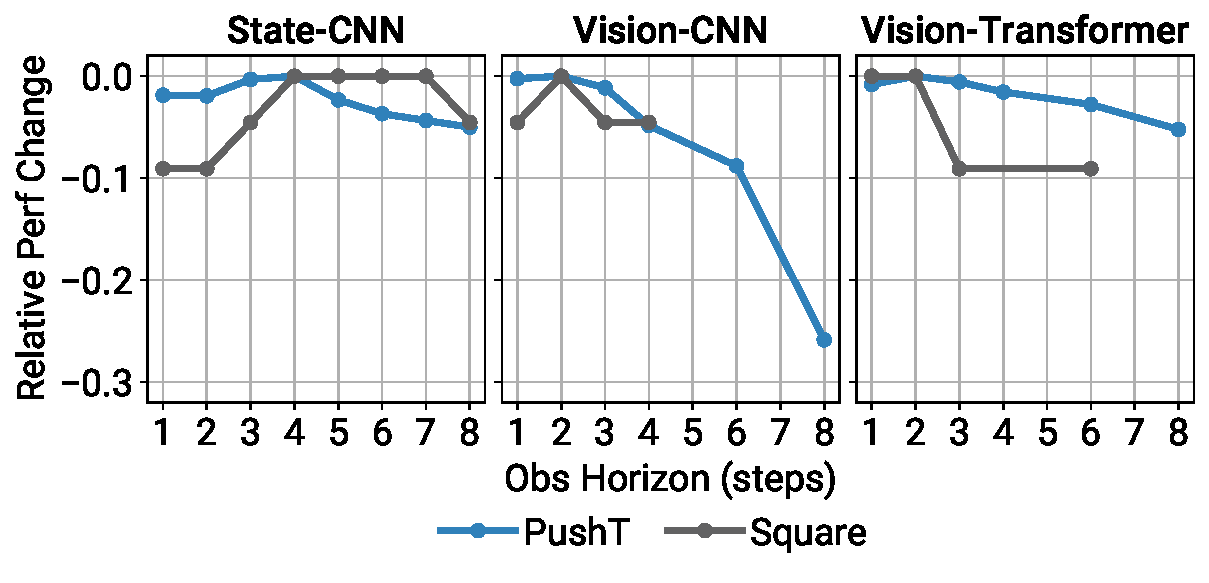
\includegraphics[width=\linewidth]{figure/obs_horizon_figure.pdf}

\vspace{-2mm}
\caption{
\textbf{Observation Horizon Ablation Study.}
\label{fig:obs_horizon_ablation}
State-based Diffusion Policy is not sensitive to observation horizon.
Vision-based Diffusion Policy prefers low but $>1$ observation horizon, with $2$ being a good compromise for most tasks.
}
\vspace{-3mm}
\end{figure}

\begin{figure}
\centering
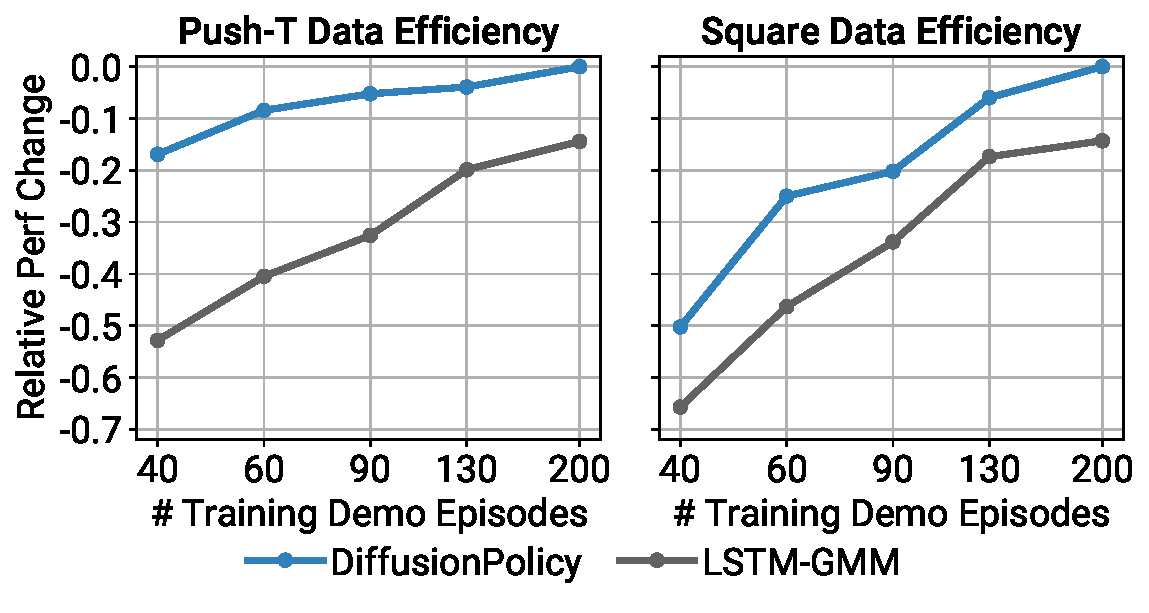
\includegraphics[width=\linewidth]{figure/sample_efficiency_figure.pdf}

\vspace{-2mm}
\caption{
\textbf{Data Efficiency Ablation Study.}
\label{fig:data_efficiency}
Diffusion Policy outperforms LSTM-GMM \cite{robomimic} at every training dataset size.
}
\vspace{-5mm}
\end{figure}

\subsection{Data Efficiency}
We found Diffusion Policy to outperform LSTM-GMM \cite{robomimic} at every training dataset size, as shown in Fig. \ref{fig:data_efficiency}.

\section{Additional Ablation Results}
\subsection{Observation Horizon}
We found state-based Diffusion Policy to be insensitive to observation horizon, as shown in Fig. \ref{fig:obs_horizon_ablation}. However, vision-based Diffusion Policy, in particular the variant with CNN backbone, see performance decrease with increasing observation horizon. In practice, we found an observation horizon of 2 is good for most of the tasks for both state and image observations.

\subsection{Performance Improvement Calculation}
For each task $i$ (column) reported in Tab. \ref{tab:table_low_dim}, Tab. \ref{tab:table_image} and Tab. \ref{tab:multi_stage} (mh results ignored), we find the maximum performance for baseline methods $max\_baseline_i$ and the maximum performance for Diffusion Policy variant (CNN vs Transformer) $max\_ours_i$. For each task, the performance improvement is calculated as $improvement_i = \frac{max\_ours_i-max\_baseline_i}{max\_baseline_i}$ (positive for all tasks). Finally, the average improvement is calculated as $avg\_improvement=\frac{1}{N}\sum^i_N improvement_i=0.46858 \approx 46.9\%$.



\section{Realworld Task Details}

\subsection{Push-T}
\subsubsection{Demonstrations}
136 demonstrations are collected and used for training. The initial condition is varied by randomly pushing or tossing the T block onto the table. Prior to this data collection session, the operator has performed this task for many hours and should be considered proficient at this task.

\subsubsection{Evaluation}
We used a fixed training time of 12 hours for each method, and selected the last checkpoint for each, with the exception of IBC, where the checkpoint with minimum training set action prediction MSE error due to IBC's training stability issue. The difficulty of training and checkpoint selection for IBC is demonstrated in main text Fig. 7.
Each method is evaluated for 20 episodes, all starting from the same set of initial conditions. To ensure the consistency of initial conditions, we carefully adjusted the pose of the T block and the robot according to overlayed images from the top-down camera.
Each evaluation episode is terminated by either keeping the end-effector within the end-zone for more than 0.5 second, or by reaching the 60 sec time limit.
The IoU metric is directly computed in the top-down camera pixel space.

\subsection{Sauce Pouring and Spreading}
\subsubsection{Demonstrations}
50 demonstrations are collected, and 90\% are used for training for each task.
For pouring, initial locations of the pizza dough and sauce bowl are varied. After each demonstration, sauce is poured back into the bowl, and the dough is wiped clean.
For spreading, location of the pizza dough as well as the poured sauce shape are varied. For resetting, we manually gather sauce towards the center of the dough, and wipe the remaining dough clean.
The rotational components for tele-op commands are discarded during  spreading and sauce transferring to avoid accidentally scooping or spilling sauce.

\subsubsection{Evaluation}
Both Diffusion Policy and LSTM-GMM are trained for 1000 epochs. The last checkpoint is used for evaluation.

Each method is evaluated from the same set of random initial conditions, where positions of the pizza dough and sauce bowl are varied. We use a similar protocol as in \textbf{Push-T} to set up initial conditions. We do not try to match initial shape of poured sauce for spreading. Instead, we make sure the amount of sauce is fixed during all experiments.

The evaluation episodes are terminated by moving the spoon upward (away form the dough) for 0.5 seconds, or when the operator deems the policy's behavior is unsafe.

The coverage metric is computed by first projecting the RGB image from both the left and right cameras onto the table space through homography, then computing the coverage in each projected image. The maximum coverage between the left and right cameras is reported.






\section{Realworld Setup Details}

\subsubsection{UR5 robot station}
\label{sec:ur5_setup}
Experiments for the \textbf{Push-T} task are performed on the UR5 robot station.

The UR5 robot accepts end-effector space positional command at 125Hz, which is linearly interpolated from the 10Hz command from either human demonstration or the policy. The interpolation controller limits the end-effector velocity to be below 0.43 m/s and its position to be within the region 1cm above the table for safety reason. Position-controlled policies directly predicts the desired end-effector pose, while velocity-controlled policies predicts the difference the current positional setpoint and the previous setpoint.

The UR5 robot station has 5 realsense D415 depth camera recording 720p RGB videos at 30fps. Only 2 of the cameras are used for policy observation, which are down-sampled to 320x240 at 10fps.

During demonstration, the operator teleoperates the robot via a 3dconnexion SpaceMouse at 10Hz.

\subsection{Franka Robot Station}
\label{sec:franka_setup}
Experiments for \textbf{Sauce Pouring and Spreading, Bimanual Egg Beater, Bimanual Mat Unrolling, and
Bimanual Shirt Folding} tasks are performed on the Franka robot station.

For the non-haptic control, a custom mid-level controller is implemented to generate desired joint positions from desired end effector poses from the learned policies. At each time step, we solve a differential kinematics problem (formulated as a Quadratic Program) to compute the desired joint velocity to track the desired end effector velocity. The resulting joint velocity is Euler integrated into joint position, which is tracked by a joint-level controller on the robot. This formulation allows us to impose constraints such as collision avoidance for the two arms and the table, safety region for end effector and joint limits. It also enables regulating redundant DoF in the null space of the end effector commands. This mid-level controller is particularly valuable for safeguarding the learned policy during hardware deployment.

For haptic teleoperation control, another custom mid-level controller is implemented, but formulated as a pure torque-controller. The controller is formulated using Operational Space Control \citet{khatib1987osc} as a Quadratic Program operating at 200 Hz, where position, velocity, and torque limits are added as constraints, and the primary spatial objective and secondary null-space posture objectives are posed as costs.
This, coupled with a good model of the Franka Panda arm, including reflected rotor inertias, allows us to perform
good tracking with pure spatial feedback, and even better tracking with feedforward spatial acceleration.
Collision avoidance has not yet been enabled for this control mode.

Note that for inference, we use the non-haptic control. Future work intends to simplify
this control strategy and only use a single controller for our given objectives.

The operator uses a SpaceMouse or VR controller input device(s) to control the robot's end effector(s), and the grippers are controlled by a trigger button on the respective device. Tele-op and learned policies run at 10Hz, and the mid-level controller runs around 1kHz. Desired end effector pose commands are interpolated by the mid-level controller. This station has 2 realsense D415 RGBD camera streaming VGA RGB images at 30fps, which are downsampled to 320x240 at 10fps as input to the learned policies.

\subsection{Initial and Final States of Bimanual Tasks}
\label{sec:bimanual_ini_fial}
The following figures show the initial and final state of four bimanual tasks. Green and red boxes indicate successful and failed rollouts respectively. Since mat and shirt are very flat objects, we used a homographic projection to better visualize the initial and final states.

\begin{figure}
    \centering
    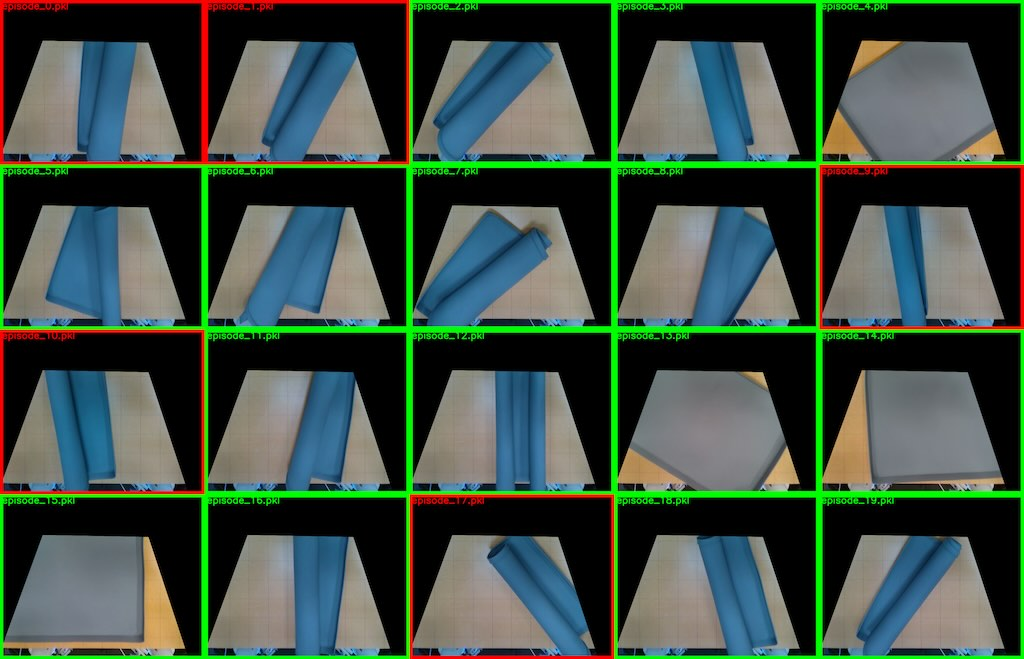
\includegraphics[width=\linewidth]{figure/ijrr24_unroll_mat_ini.jpg}
    \caption{Initial states for Mat Unrolling}
    \label{fig:unroll_mat_ini}
    \centering
    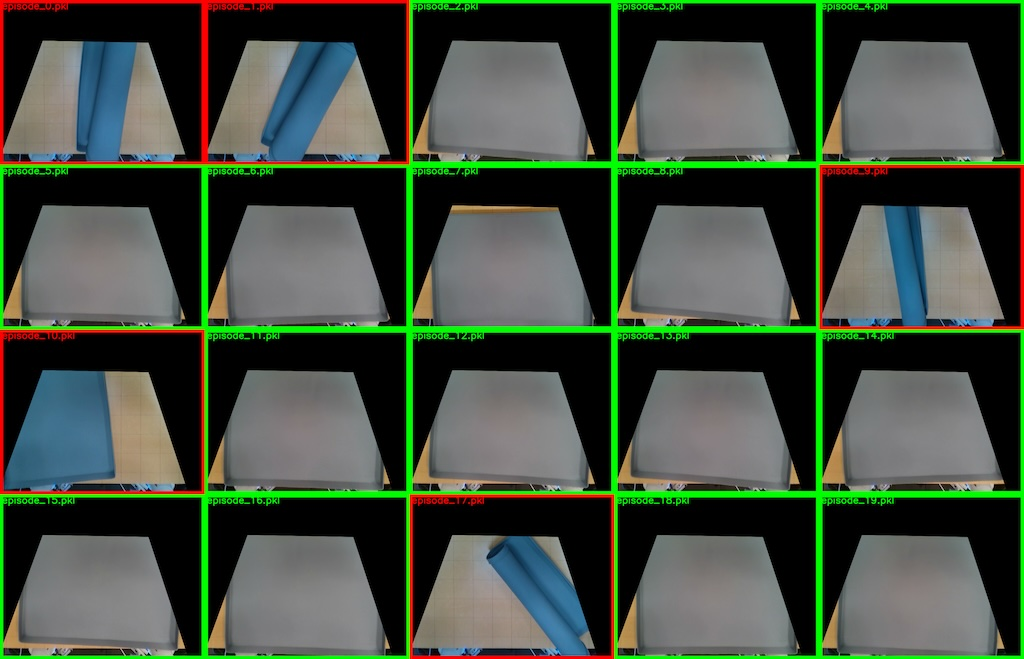
\includegraphics[width=\linewidth]{figure/ijrr24_unroll_mat_last.jpg}
    \caption{Final states for Mat Unrolling}
    \label{fig:unroll_mat_last}
\end{figure}


\begin{figure}
    \centering
    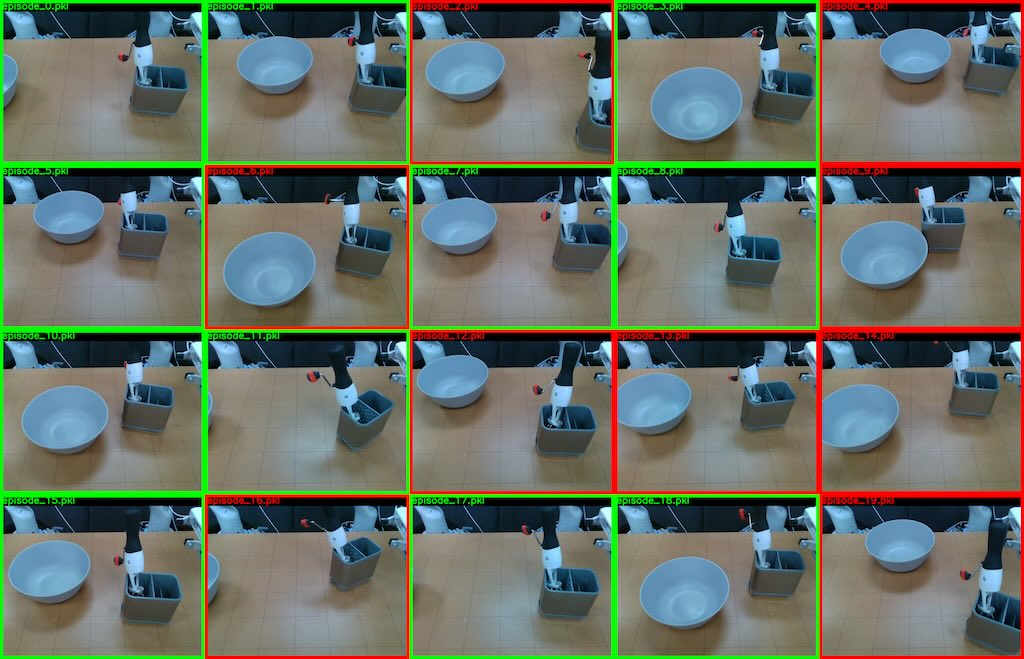
\includegraphics[width=\linewidth]{figure/ijrr24_egg_beater_ini.jpg}
    \caption{Initial states for Egg Beater}
    \label{fig:egg_beater_ini}
    \centering
    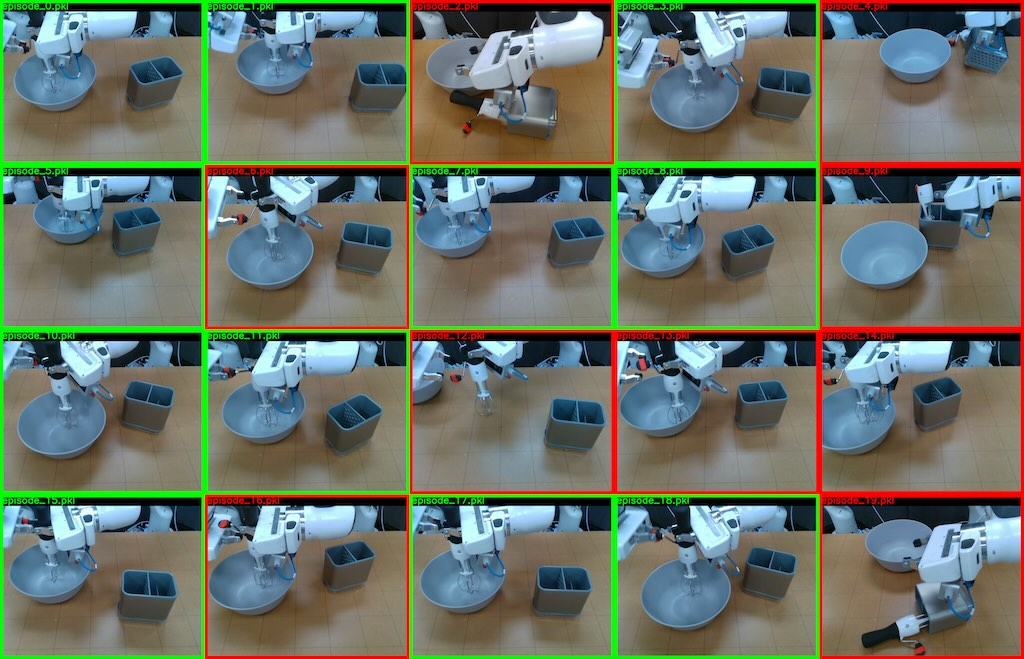
\includegraphics[width=\linewidth]{figure/ijrr24_egg_beater_last.jpg}
    \caption{Final states for Egg Beater}
    \label{fig:egg_beater_last}
\end{figure}


\begin{figure}
    \centering
    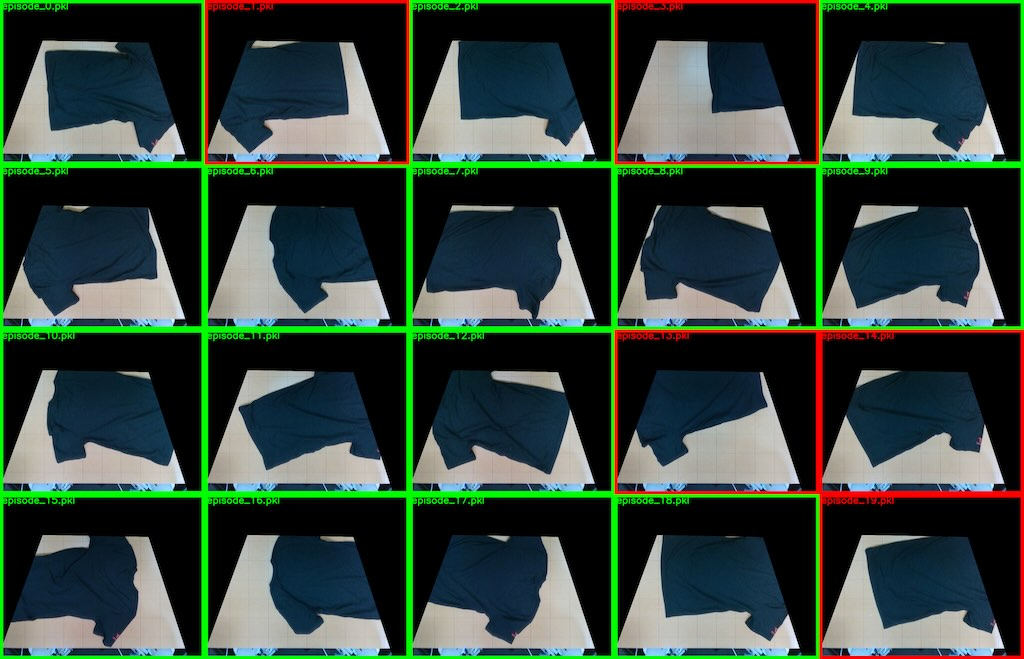
\includegraphics[width=\linewidth]{figure/ijrr24_fold_shirt_ini.jpg}
    \caption{Initial states for Shirt Folding}
    \label{fig:fold_shirt_ini}
    \centering
    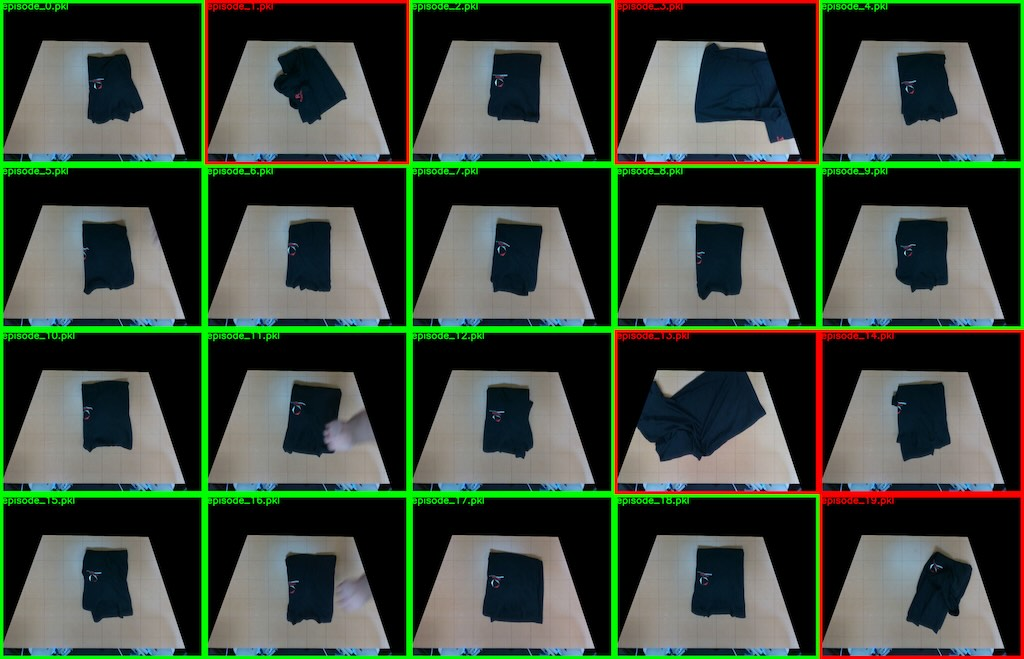
\includegraphics[width=\linewidth]{figure/ijrr24_fold_shirt_last.jpg}
    \caption{Final states for Shirt Folding}
    \label{fig:fold_shirt_last}
\end{figure}
